%\documentclass[aspectratio=43]{beamer}
\documentclass[t]{beamer}
\usetheme{ffmodern}  %% Themenwahl

\usepackage[ngerman]{babel} 
\usepackage[T1]{fontenc}    % richtige Silbentrennung
\usepackage[utf8]{inputenc} % Umlaute etc.!
\usepackage{eurosym}
\usepackage{tikz}
\usepackage{pgffor}

\usetikzlibrary{arrows,decorations.pathmorphing,backgrounds,fit,positioning,shapes.symbols,chains}

%1

\title{Freifunk Helgoland}
\author{hamburg.freifunk.net}
\date{2015-Jan-23}
\license{CC-BY-3.0}

%2
\begin{document}
\maketitle

\begin{frame}{Was ist freifunk?}
	\begin{itemize}
		\item Initiative für freie, offene, kostenlose Netzwerke
		\item Steht jedem offen, als Nutzer oder Anbieter
		\item Wird von den Menschen betrieben, die es nutzen
		\item Nicht kommerziell
		\item Nutzt freie, quelloffene Programme
		\item Netzneutral - keine Manipulation der Datenströme		
	\end{itemize}
\end{frame}

%2
\begin{frame}{Verbreitung}
	\begin{columns}
		\begin{column}{0.6\textwidth}
			\begin{itemize}
				\item In  \href{http://freifunk.net/wie-mache-ich-mit/community-finden/}{150 Orten} gibt es bereits Freifunknetze mit mehr als 8400 Zugangspunkten
				\item Kooperation mit Stadtverwaltungen von Berlin \& Lübeck
			\end{itemize}
		\end{column}
		\begin{column}{0.4\textwidth}
			\begin{center}
				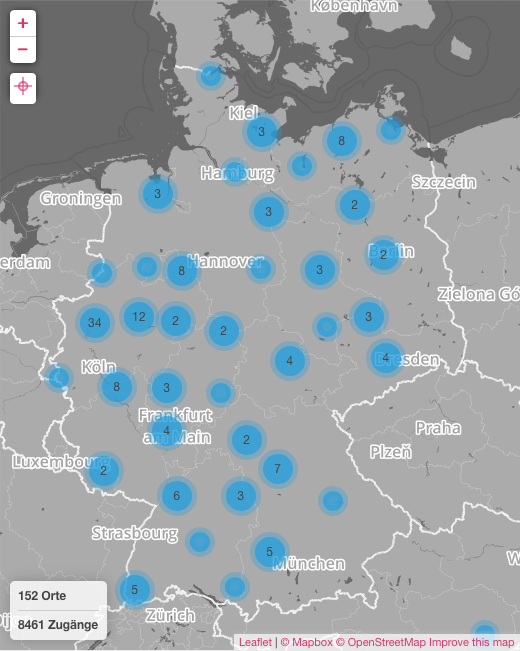
\includegraphics[width=\textwidth]{Bilder/Deutschlandkarte}
			\end{center}
		\end{column}
	\end{columns}
\end{frame}

%9
\begin{frame}{Knotenkarte von Hamburg}
	\begin{center}
		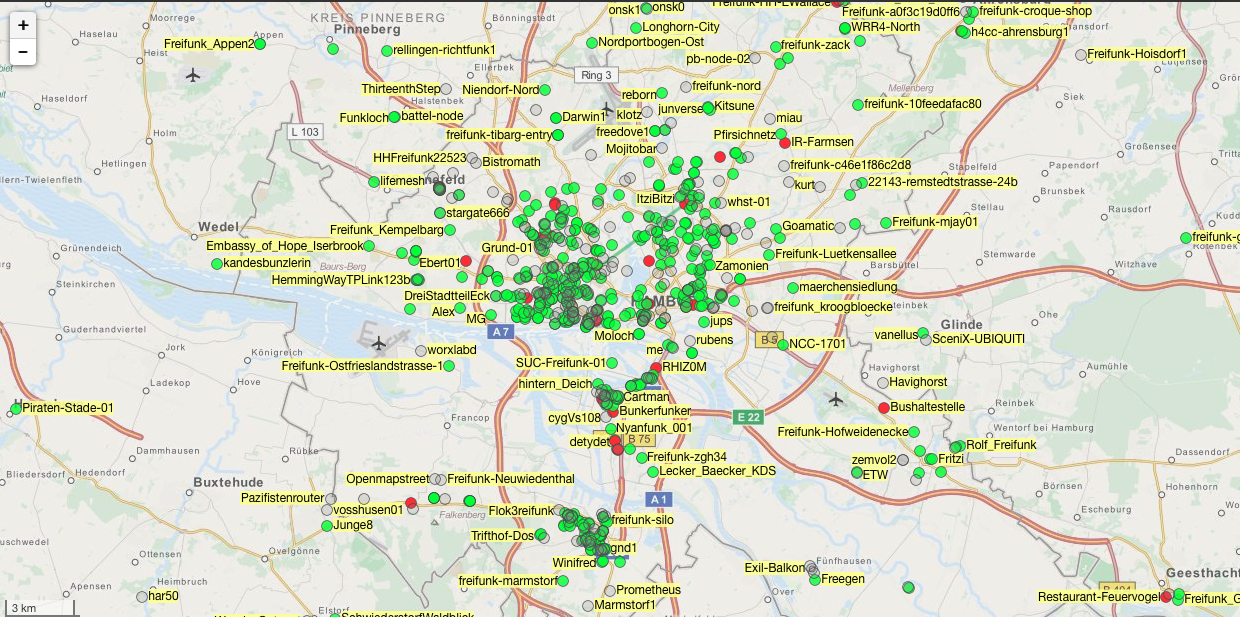
\includegraphics[width=1\textwidth]{Bilder/knotenkarte1}
	\end{center}
\end{frame}

%3
\begin{frame}{Freifunkknoten}
	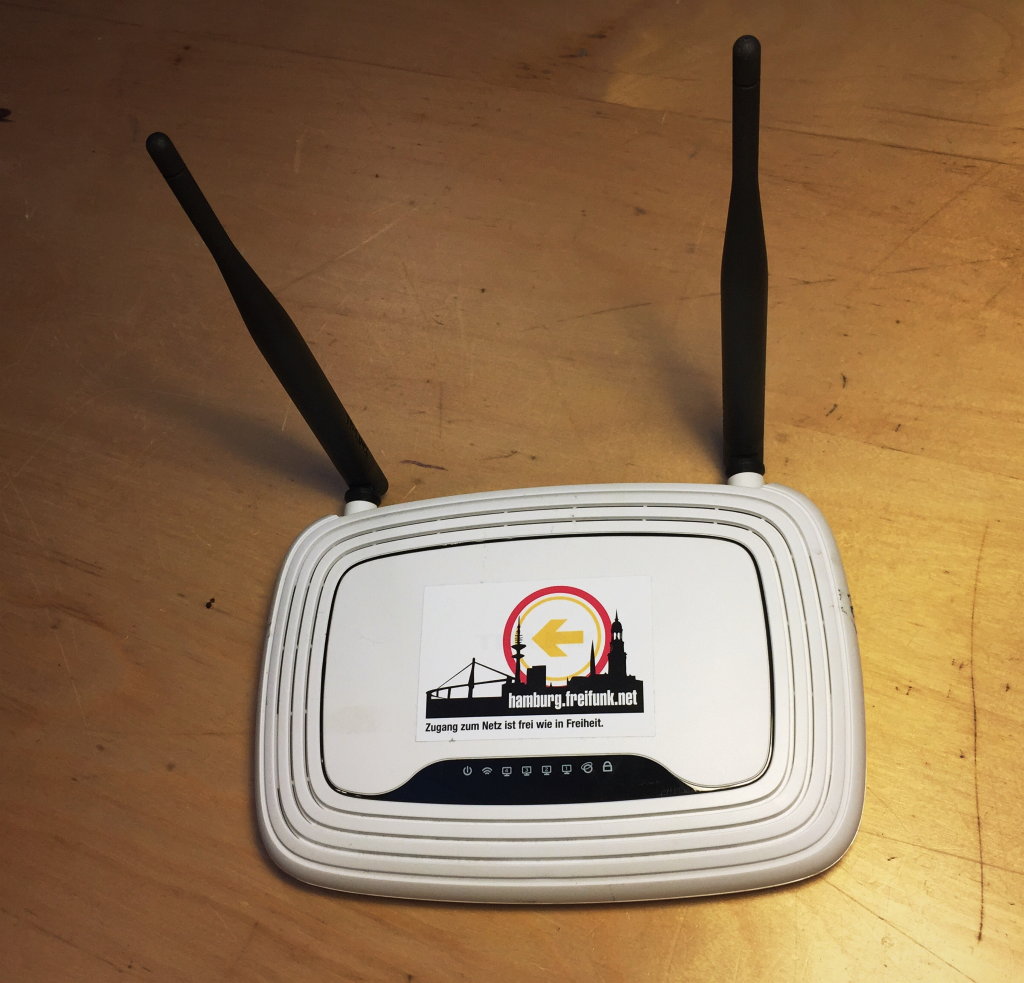
\includegraphics[width=.6\textwidth]{Bilder/841}
\end{frame}

\foreach \index in {1, ..., 4} 
{
    \begin{frame}{Das Netzwerk}
        \centering \includesvg[width=9cm]{netz-\index}
    \end{frame}
}


%10
\begin{frame}{Sicherheit}
	\begin{itemize}
		\item Wie bei allen offenen WLANs, ist die Funkstrecke zum Zugangspunkt unverschlüsselt
		\item Wie sonst im Netz auch, sollte nach Möglichkeit Ende-zu-Ende-Verschlüsselung genutzt werden
		\item Freifunk und Heim- / Firmennetz sind getrennt
	\end{itemize}
\end{frame}


%11
\begin{frame}{Haftung}
	\begin{itemize}
		\item Keine Haftung für Knotenbetreiber
		\item Aller Internetverkehr geht durch die Gateways. Diese sind nach TMG\S8 von Haftung befreit.
		\item Wir nehmen die gesetzlichen Vorschriften wörtlich: Wir sammeln keine Daten.
	\end{itemize}
\end{frame}


%13
\begin{frame}{Richtfunknetz}
	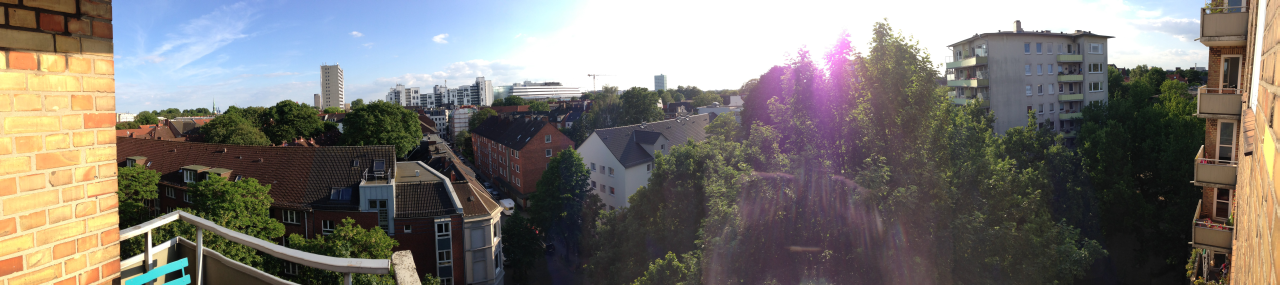
\includegraphics[width=\textwidth]{Bilder/esmarch95}
	\begin{columns}
		\begin{column}{0.7\textwidth}
			\begin{itemize}
				\item Möglichkeit das Netz durch Richtfunkstrecken von Haus zu Haus weiter zu leiten
				\item Erhöhte Standorte (z.B. Kirchturm) sind von Vorteil
			\end{itemize}
		\end{column}
		\begin{column}{0.3\textwidth}
			\begin{center}
				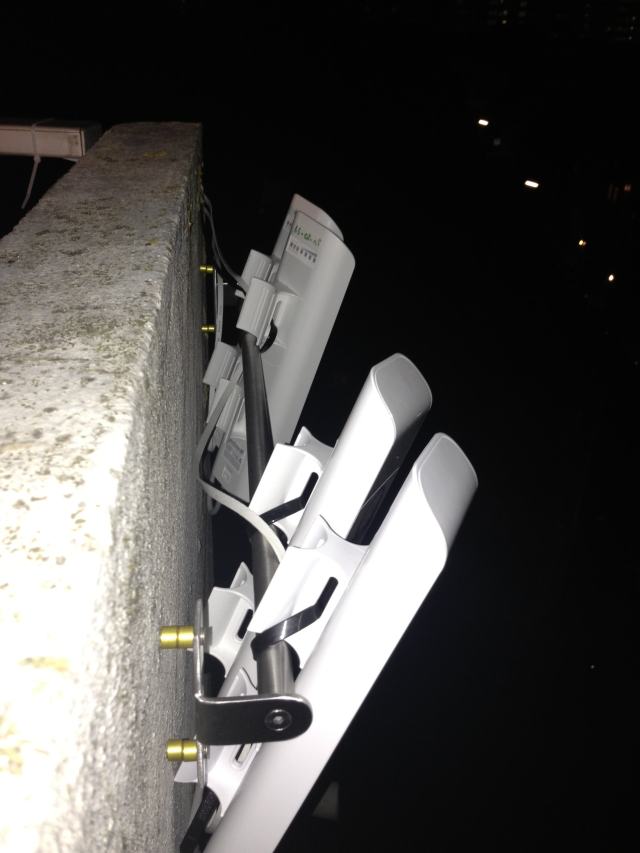
\includegraphics[width=.8\textwidth]{Bilder/esmarch95-2}
			\end{center}
		\end{column}
	\end{columns}
	
\end{frame}

%12
\begin{frame}{Dienste}
	\begin{itemize}
		\item Internet (IPv4 \& IPv6)
		\item Inselweites Intranet (IPv4 \& IPv6)
		\item Verbindungen zu anderen Städten und Netzwerken sowie deren Diensten (IP-Telefonie, Videochat...)
		\item Jeden Dienst den man selbst gerne anbieten möchte
	\end{itemize}
\end{frame}


%
\begin{frame}{\hl{Starthilfe} aus Hamburg}
	\begin{itemize}
		\item Firmware
		\item Gatewaybetrieb
		\item Geräte
		\item Wissenstransfer
	\end{itemize}
\end{frame}


%
\begin{frame}{Was bringt Helgoland mit?}
	\begin{itemize}
		\item Knotenstandorte
		\item Fixe Ansprechpartner, die bereit sind sich in die Technik einzuarbeiten
		\item helgoland.freifunk.net
		\item Bringt Euch selbst ein. Das Netz lebt ausschliesslich von ehrenamtlichen Engagement!
	\end{itemize}
\end{frame}


%17
\begin{frame}{}
	\begin{columns}
		\begin{column}{1\textwidth}
			\begin{itemize}
				\item Netz: hamburg.freifunk.net
				\item Ansprechpartner: Alexander Bernhardt 
				\item Mail: bernhardt@hauptsache.net
		\end{itemize}
			\begin{center}
				
\includegraphics[width=0.2\textwidth]{Bilder/cc-by}
			\end{center}
		\end{column}
	\end{columns}
\end{frame}

\end{document}